%%%%%%%%%%%%%%%%%%%%%%%%%%%%%%%%%%%%%%%%%%%%%%%%%%%%%%%%%%%%%%%%%
% Dissertacao de Mestrado / Dept Fisica, CFM, UFSC              %
% Andre@UFSC - 2011                                             %
%%%%%%%%%%%%%%%%%%%%%%%%%%%%%%%%%%%%%%%%%%%%%%%%%%%%%%%%%%%%%%%%%

%:::::::::::::::::::::::::::::::::::::::::::::::::::::::::::::::%
%                                                               %
%                          Capítulo 3                           %
%                                                               %
%:::::::::::::::::::::::::::::::::::::::::::::::::::::::::::::::%

%***************************************************************%
%                                                               %
%                         Crossmatch                            %
%                                                               %
%***************************************************************%

\chapter{Crossmatch entre \SDSS/\starlight e \galex}
\label{sec:Crossmatch}

% TODO: Crossmatch - intro do capítulo.
TODO: Crossmatch - intro do capítulo.

\section{\SDSS {\em SkyServer} e {\em CasJobs}}
Um dos maiores responsáveis pela promoção do uso de bancos de dados relacionais
na astronomia é o projeto {\em Sloan Digital Sky Survey} (\SDSS). Inicialmente o
\SDSS utilizou um {\em sistema de gerenciamento de banco de dados orientado a
objetos} (OODBMS, na sigla em inglês). Após pouco mais de um ano a abordagem se
mostrou inadequada: entre os principais problemas, uma linguagem de {\em query}
inadequada e performance ruim. O motivo, segundo \cite{Thakar2004}, foi a
incapacidade da empresa desenvolvedora do OODBMS em prover novas funcionalidades
requisitadas pelo projeto e correção de {\em bugs}, bem como em acompanhar o
crescimento da performance do {\em hardware}.

Todo o banco de dados do \SDSS foi migrado para um {\em sistema de gerenciamento
de banco de dados relacional} (RDBMS, na sigla em inglês). RDBMS pode ser
considerado o padrão da indústria. Praticamente todas as linguagens de
programação tem bibliotecas de interface às implementações de RDBMS comerciais
mais comuns (Oracle, IBM e Microsoft). Há uma diversidade de ferramentas para
desenvolvimento e gerenciamento de RDBMS. E talvez o maior benefício de todos, o
acesso aos dados é feito utilizando uma linguagem padronizada: Simple Query
Language (SQL) \citep{Codd1970}. A migração dos dados do \SDSS para um RDBMS
comercial implicou num aumento significativo da performance do acesso aos dados,
e resultou no desenvolvimento do {\em SkyServer}\footnote{SkyServer:
\url{http://skyserver.sdss.org/}}.

O {\em SkyServer} é um {\em website} que provê acesso aos dados armazenados no
banco de dados do \SDSS \citep{Szalay2002}. O acesso mais simples pode ser feito
através de um atlas de locais famosos {\em famous places}, que mostra imagens
coloridas de objetos celestes conhecidos. Há formulários para buscas mais
sérias, gerando coleções de imagens, espectros e tabelas de dados. No {\em
SkyServer} é possível fazer buscas avançadas utlizando SQL, embora haja limites
de tempo de execução e de quantidade de objetos retornados. Esta limitação é
contornada através do sistema {\em CasJobs}, que será tratado adiante.

É importante ressaltar que o {\em SkyServer} permite (ou mais adequadamente,
encoraja) a criação de {\em mirrors}\footnote{{\em Mirror}: Espelho, em inglês.
Clone de um website.}. Todo o banco de dados do \SDSS e o código fonte do {\em
SkyServer} está disponível no próprio {\em website} do {\em SkyServer}. Há um
clone do banco de dados do {Data Release} 8 do \SDSS no servidor {\em CasJobs}
do \starlight \footnote{{\em CasJobs} do \starlight:
\url{http://casjobs.starlight.ufsc.br/casjobs/}}.

\subsection{{\em CasJobs}}
% TODO: Apresentar o Casjobs.
\cite{Li2008}.
\begin{verbatim}
Catalog Archive Server Jobs (CasJobs) is an asynchronous query
workbench service that lets users run unrestricted SQL queries against
scientific catalog archives. After running queries in batch mode, users can save
their results to a personal database called MyDB before downloading them,
letting users manage their query workloads, results, and histories without
causing network overload.

CasJobs has become the mainstay and workhorse of the SDSS data-access system.
It’s in use at SDSS mirror sites worldwide and has also been adapted for
non-SDSS astronomical archives, such as Galaxy Evolution Explorer (GALEX),
Palomar Quest, and the upcoming Panoramic Survey Telescope and Rapid Response
System (Pan-STARRS) PS1 archive, as well as for non-astronomy applications that
contain hydrology sensor data such as AmeriFlux. The technologies that CasJobs
employs—asynchronous query execution and personal server-side database
access—are universally applicable and inescapable for query management in very
large online databases.
\end{verbatim}

\section{Banco de dados do \starlight}
% TODO: Construção do banco de dados do starlight.
TODO: Construção do banco de dados do starlight Starlight gera dados em arquivos
texto. São gigabytes de dados. Tratável para uso pessoal, mas não é muito viável
a distribuição.

Importação para o sql server?.

\subsection{Estrutura do banco de dados}
% TODO: Estrutura banco de dados do starlight.
TODO: Estrutura banco de dados do starlight.

% TODO: Adicionar figura - esquema BD starlight.
\begin{figure}
	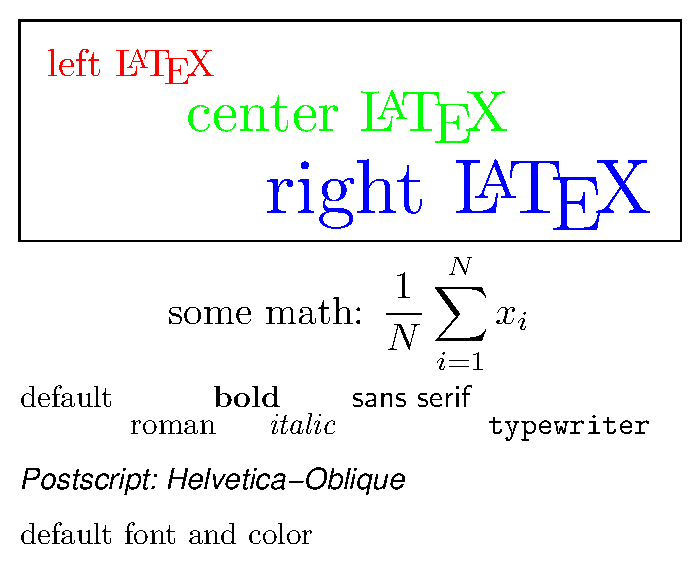
\includegraphics[width=0.5\textwidth]{figuras/test.eps}
	\caption[Esquema do banco de dados do \starlight.]
	{Esquema do banco de dados do \starlight.}
	\label{fig:EsquemaBDStarlight}
\end{figure}

\subsection{Amostra do \starlight}
\label{sec:Crossmatch:AmostraStarlight}
% TODO: Definir a amostra inicial do starlight. FIXME: Explicar o que é uma
% chave primária.
A amostra de galáxias do \starlight contém $926246$ espectros do \SDSS. A
identificação de cada espectro é feita através de um tripleto: a data juliana
média da observação ({\tt MJD}, {\em Mean Julian Date}), a identificação da
placa de suporte das fibras ópticas ({\tt Plate}) e a identificão da fibra
utilizada para a obtenção do espectro ({\tt FiberID}). Este tripleto ({\tt MJD},
{\tt Plate}, {\tt FiberID}) identifica unicamente um espectro. Porém, é mais
conveniente (e eficiente) ter um identificador único{\footnote{Chave primária
\fixme}} para os registros num banco de dados. No caso do \SDSS, a tabela de
espectros ({\tt SpecObjAll}) tem um identificador chamado {\tt SpecObjID}.

% TODO: Adicionar figura - esquema simplificado da BD do SDSS.
\begin{figure}
	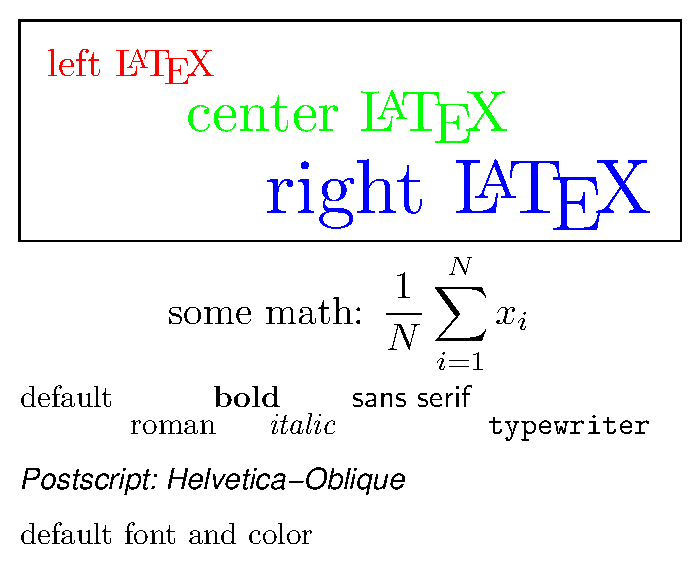
\includegraphics[width=0.5\textwidth]{figuras/test.eps}
	\caption[Esquema do banco de dados do \SDSS.]
	{Esquema do banco de dados do \SDSS.}
	\label{fig:EsquemaSDSS}
\end{figure}

% FIXME: Citação para cobertura do céu do SDSS.
Além de espectros, o banco de dados do \SDSS (figura \ref{fig:EsquemaSDSS})
contém fotometria de $1/4$ do céu.\citneed Os objetos com dados de fotometria
também tem um identificador único, {\tt ObjID}. Existe uma coluna na tabela de
espectros chamada {\tt BestObjID}, que aponta para o registro de fotometria
(tabela {\tt PhotoObjAll}) mais provável para cada espectro. É importante
salientar que nem todo espectro tem um {\tt BestObjID} definido.

A tabela de índices da amostra de galáxias do \starlight (esquema na figura
\ref{fig:TabelaAmostraStarlight}) contém inicialmente os tripletos [{\tt MJD},
{\tt Plate}, {\tt FiberID}]. Dentro do ambiente {CasJobs} do \SDSS
DR7\footnote{{\em CasJobs} \SDSS DR7 - \url{http://casjobs.sdss.org/CasJobs/}} a
tabela tem os valores de {\tt SpecObjID} e {\tt BestObjID} prenchida através da
execução da {\em query} mostrada na figura \ref{fig:AtualizaObjIds}. Entre os
objetos na amostra do \starlight, $622$ objetos não tem a sua contraparte
fotométrica.

% TODO: Adicionar figura - Tabela amostra do starlight.
\begin{figure}
	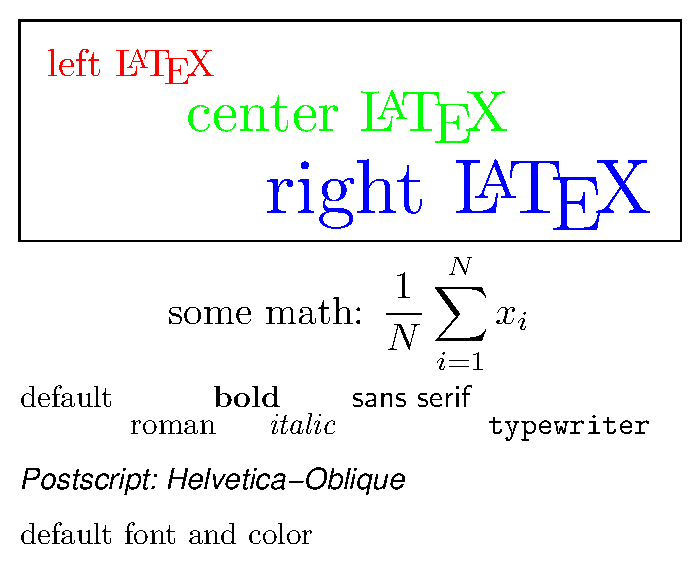
\includegraphics[width=0.5\textwidth]{figuras/test.eps}
	\caption[Esquema da tabela de índices da amostra do \starlight.]
	{Esquema da tabela de índices da amostra do \starlight. Os tipos de dados são
	referentes à implementação do banco de dados.}
	\label{fig:TabelaAmostraStarlight}
\end{figure}

\begin{figure}
	\begin{Verbatim}[commandchars=\\\{\}]
	\textbf{UPDATE} sample
		\textbf{SET} SpecObjID=so.SpecObjID, ObjID=so.BestObjID
	\textbf{FROM} sample s2 \textbf{INNER JOIN} DR7..SpecObjAll so
		\textbf{ON} so.MJD=s2.MJD
		\textbf{AND} so.Plate=s2.Plate
		\textbf{AND} so.FiberID=s2.FiberID
	\end{Verbatim}
	\caption
	[{\em Query} para atualizar os índices da amostra de galáxias do
	\starlight.]
	{Atualização dos índices da amostra de galáxias do \starlight. A {\em query}
	foi executada no {\em CasJobs} do \SDSS DR7 para obter {\tt SpecObjID} e {\tt
	BestObjID} dado o tripleto [{\tt MJD}, {\tt Plate}, {\tt FiberID}].}
	\label{fig:AtualizaObjIds}
\end{figure}


\section{Crossmatch \SDSS/\galex}
% TODO: Crossmatch SDSS/GALEX.
TODO: Crossmatch SDSS/GALEX. \cite{Budavari2009}.

\subsection{Indexação HTM}
% TODO: Indexação HTM.
TODO: Indexação HTM. \cite{Kunszt2000}.
\begin{verbatim}
The Spatial Indexing used in the Sloan
Digital Sky Survey (SDSS) Science Archive divides the spherical surface into
triangles in a hierarchical scheme resulting in roughly equal surface areas at
each level, which is a big advantage over other schemes. The location of a point
on the sky may be given by the unique index id to any level, refining it with
each step. This naming scheme is being used successfully in other catalogs, too,
like GSC-II and GAIA. The use of the Spatial Index in the SDSS is two-fold, a
level-5 index is used to partition the bulk data, and a high-resolution level-14
index id is assigned to each data point to enable quick lookup and proximity
searches. Use of this indexing scheme in more catalogs will enormously simplify
cross-matching of objects. Using a new computing paradigm, we recently realized
a quantum leap in performance that makes this scheme competitive with
bit-interleaving and requires very little memory. The Flux-space Indexing used
is a traditional k-d tree. The space is 5 dimensional, 5 being the number of
SDSS-filters. The specialization to astronomical data has been achieved by
modeling the location of the main branch in this space and applying the k-d tree
subdivisions only to its confined area. The outliers are indexed separately.
Most of the interesting data points come directly from the outlier part of the
index, with no additional analytical effort. Additionally, the key-lookup index
feature of object-oriented databases is exploited for much-used parameters like
flags.
\end{verbatim}

\subsection{Análise de completeza}
% TODO: Análise de completeza do crossmatch SDSS/GALEX
TODO: Análise de completeza do crossmatch SDSS/GALEX


\section{Definição das amostras \SDSS/\starlight e \galex}
\label{sec:Crossmatch:DefAmostras}
% TODO: Definição das amostras a serem usadas no próximo cap. (MGS e LRG).

% TODO: Como foi feito o match.

% TODO: Adicionar figura - tabela xSDSSDR7.
\begin{figure}
	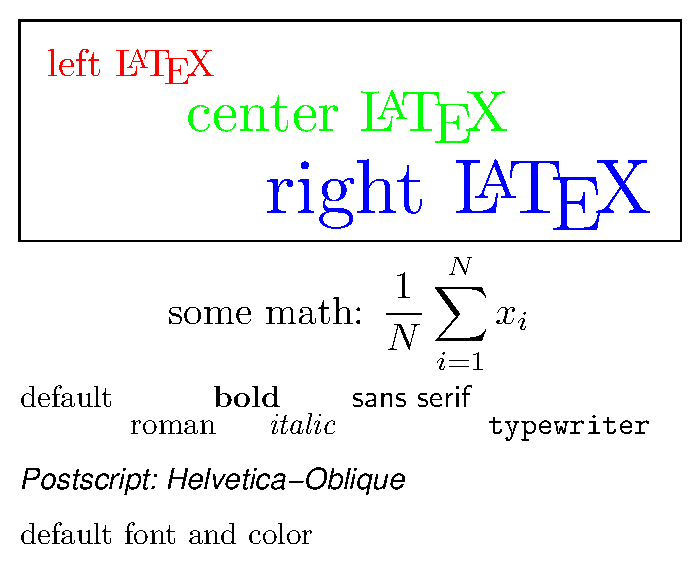
\includegraphics[width=0.5\textwidth]{figuras/test.eps}
	\caption[Esquema da tabela de {em crossmatch} entre objetos do \galex e do
	\SDSS.]
	{Esquema da tabela de {\em crossmatch} entre objetos do \galex e do
	\SDSS.}
	\label{fig:TabelaxSDSSDR7}
\end{figure}

% FIXME: Corrigir caption da figura do match AIS.
\begin{figure}
	\begin{Verbatim}[commandchars=\\\{\}]
	\textbf{SELECT INTO} mydb..galex_ais
		s.objid \textbf{AS} sdssobjid, x.objid \textbf{AS} galexobjid,
		s.mjd, s.plate, s.fiberid,
		g.nuv_mag, nuv_magErr,
		g.fuv_mag, g.fuv_magErr,
		g.e_bv,
		g.band,
		x.distance,
		pe.nexptime,
		pe.fexptime
	\textbf{FROM} mydb..sample s
	\textbf{LEFT JOIN} xSDSSDR7 x
		\textbf{ON} s.objid = x.sdssobjid
		\textbf{AND} x.distanceRank=1
		\textbf{AND} x.reverseDistanceRank=1
		\textbf{AND} x.multipleMatchCount=1
		\textbf{AND} x.reverseMultipleMatchCount=1
	\textbf{LEFT JOIN} photoobjall g
		\textbf{ON} g.objid = x.objid
	\textbf{LEFT JOIN} photoextract e
		\textbf{ON} e.photoextractid=g.photoextractid
	\textbf{WHERE} e.mpstype='AIS'
	\end{Verbatim}
	\caption[{\em Query} para o {\em match} entre os objetos da amostra do
	\starlight e \galex AIS.]
	{{\em Query} para o {\em match} entre os objetos da amostra do \starlight e
	\galex AIS. A mesma {\em query} foi usada para o MIS, trocando apenas o nome da
	tabela para {\tt galex\_mis} e modificando a última linha para {\tt
	e.mpstype='MIS'}.}
	\label{fig:QueryMatchAIS}
\end{figure}


% TODO: Alguma estatística.


\section{Correções na fotometria UV}
\label{sec:Crossmatch:Correcoes}

\subsection{K-correct}
% TODO: K-correction

\subsection{Poeira}
% TODO: Correção por poeira etc.


%% End of this chapter
